\section{Container}
\label{sec:grundlagen:container}

Im Gegensatz zu bewährten Virtualizierungsumgebungen wie VMWare und KVM, 
die eigene Ressourcen wie CPU, RAM und einen Linux Kernel virtualisieren,
nutzen Container die Ressourcen des Hostsystems. 
Alle Container nutzen den selben Kernel und Isolation ist dort implementiert.
Container sind deshalb sehr ressourceneffizient, da nicht für jede Anwendung ein eigenes
Betriebssystem genutzt werden muss \cite{Kane2018}.

\begin{figure}
  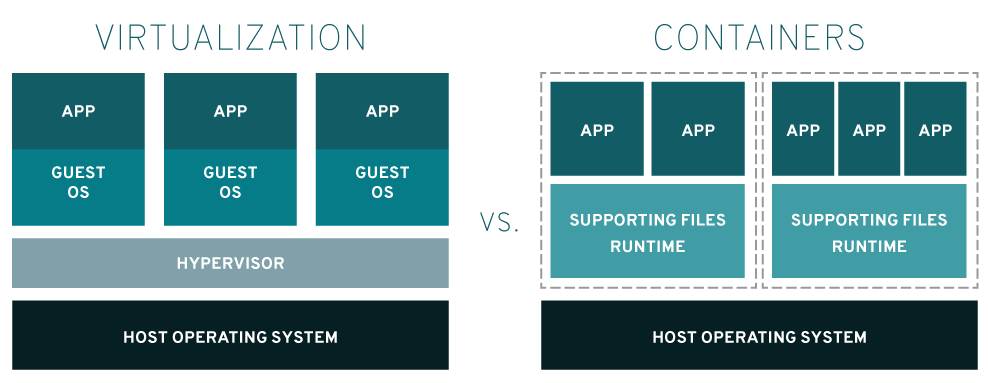
\includegraphics[width=\textwidth]{gfx/chapters/2_grundlagen/virtualization-vs-containers.png}
  \label{fig:container:vergleich}
  \caption{Virtualization vs. Container Technologie}
  \source{\cite{Kane2018}}
\end{figure}